\documentclass[english,12pt,a4paper,final]{article}
\usepackage[T1]{fontenc}
\usepackage[left=2cm, right=2cm, top=2cm, bottom=2cm]{geometry}
\usepackage{amssymb,graphicx,amsfonts,amsthm, tikz, listings}
\usepackage{bookman}
\usepackage{babel}
\usetikzlibrary{shapes.geometric, arrows}
\begin{document}
	\begin{titlepage}
		\centering
		% TODO: \usepackage{graphicx} required
		
\includegraphics[width=0.15\textwidth]{logounesa.png}\par\vspace{1cm}
		{\large\textsc{Bachelor Degree of Mathematics} \par}
		\vspace{1cm}
		{\Large \textsc{Assignment Report}\par}
		\vspace{1.5cm}
		{\huge\bfseries Programming Language\par}
		{\Large \textsc{4420102177}\par}
		\vspace{2cm}
		Oleh:\\
		{\Large\itshape Type your name\par}
		22030214XXX\\
		MA - 2022X
		\vfill
		Supervised by\par
		Dimas Avian \textsc{Maulana}, M.Si.\\
		
		\vfill
		Teaching Assistant:\par
		Elena Merdekawati Putri Haries
		\vfill
		% Bottom of the page
		{\large \today\par}
	\end{titlepage}
	\section{Problem Statement}
	Describe the problem you solve today
	\section{Flowchart}
	Make a flowchart based on problem statement. Here's an example:
		\begin{figure}[h!]
			\tikzstyle{startstop} = [rectangle, rounded corners=0.5cm, minimum width=2.5cm, minimum height=1cm, text centered, draw=black]
			\tikzstyle{io} = [trapezium, trapezium stretches=true, trapezium left angle=70,  trapezium right angle=110, minimum height=1cm, text centered, draw=black]
			\tikzstyle{process} = [rectangle, minimum width=3cm, minimum height=1cm, text centered, draw=black]
			\tikzstyle{decision} = [diamond, minimum height=1cm, aspect=2.5, text centered, draw=black]
			\tikzstyle{arrow} = [ultra thick,->,>=stealth]
			\centering
			\begin{tikzpicture}[node distance=2.25cm]
				\node (start) [startstop] {Start};
				\node (in) [io, below of=start] {Stock Data};
				\node (pro2) [decision, below of=in] {Input Parameter};
				\node (pro3) [process, below of=pro2] {Compute $dt, u, d, p, v_{es}$ and $S_{ij}$};
				\node (pro4) [process, below of=pro3] {Compute the call option at maturity};
				\node (pro5) [process, below of=pro4] {Do the countdown as Binomial method to obtain $f_{0,0}$};
				\node (stop) [startstop, below of=pro5] {End};
				
				\draw [arrow] (start) -- (in);
				\draw [arrow] (in) -- (pro2);
				\draw [arrow] (pro2) -- (pro3);
				\draw [arrow] (pro3) -- (pro4);
				\draw [arrow] (pro4) -- (pro5);
				\draw [arrow] (pro5) -- (stop);		
			\end{tikzpicture}
			\caption{Flow chart}
		\end{figure}
	\section{\textit{Source Code}}
	Type the source code here. This is the example of source code:
	\lstinputlisting[language=python]{epidemiology.py} %ganti epidemiology.py dengan file Anda
	
	\section{Screenshots of Running Programme}
	\begin{figure}
		\centering
		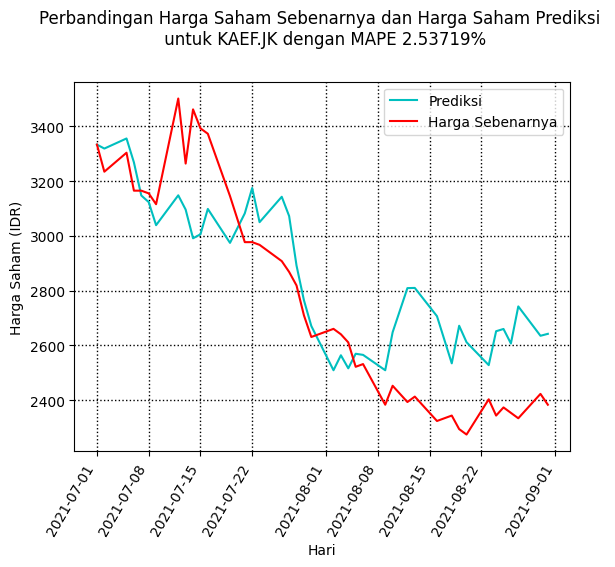
\includegraphics[width=\linewidth]{KAEF}
		\caption{Output of the programme with xxx}
		\label{fig:kaef}
	\end{figure}
	
	\section{Description}
	Give some descriptions on the problem you solve.
	
	\begin{thebibliography}{9} 
		\bibitem{Azuela} Mariano Azuela, \textit{The Underdogs: A Novel of the Mexican Revolution}, trans. Beth Jorgensen (New York: The Modern Library, 2002). 
	\end{thebibliography}
\end{document}